\section{Introducing Rust for Scientific Software}\label{chpt:1:sec:2}

Rust is a modern system-level programming language, introduced by Mozilla in 2015 as a direct replacement for C/C++, and is bundled with features that favour safety for shared memory programming. Having identified it as a suitable candidate for our programming environment, we list a few of its key benefits in this section.

Fortran and C/C++ have have continued to dominate high-performance scientific computing applications, the main criticism of these languages for academic software is their relatively poor developer experience. C/C++ especially has significant flexibility in the compilers, documentation, build systems and package managers that developers can choose to work with, as well as support for multiple paradigms and a growing syntax. Rust stands in contrast to this with a single centrally supported runtime system, Cargo, with common standards for testing and documentation. Additionally, there is only a single Rust compiler, rustc. This inflexibility, in addition to a strongly preferred way of organising Rust code via its Traits system, makes Rust libraries significantly more uniform and readable than corresponding C++ code. Indeed installing a Rust library, or building a binary, is often as simple as running a single command from a terminal, or adding a single line to a TOML dependency file.

The lack of a uniform building and packaging standards in C/C++ means that some projects go as far as to implement a custom build system, such as the Boost library \cite{boostbuild2022github}. With the exception of Fortran, which has made recent strides to develop a standardised modern package manager and build system, inspired by Rust's Cargo \cite{fpm2022github}, C and C++ do not have a single officially supported package manager or build system. The resulting landscape is a multitude of package managers \cite{spack2022github, vcpkg2022github, conan2022github} and build systems \cite{meson2022github, bazel2022github, scons2022github} a few of which we have cited here, all of which replicate each others functionality, none of which are universally accepted or implemented across projects nor officially supported by the C++ software foundation. Figure (\ref{fig:chpt:1:sec:2:builds}) provides an overview of a few of the myriad approaches taken in other languages. To manage this complexity, builds are often defined using a metabuild system, most commonly CMake. CMake is a scripting language, and as a meta build system it takes a specification of local and third party dependencies and hardware targets, and generates Makefiles. CMake gives developers a great deal of flexibility, it is multi-platform, and language agnostic, however it is not straightforward to maintain projects as the number of dependencies grows. Indeed, there is a significant body of literature discussing best practices with CMake \cite{scott2018professional}. However, CMake is not responsible for downloading and installing third party packages or verifying their relative compatibility, implementing its best practices is again left to users. Cargo's relative simplicity mirrors the simple build systems of high-level languages such as Python or Julia, and removes one of the main causes of development pain when working with compiled languages, and makes it significantly easier for small teams to publish software that can be easily deployed by downstream users regardless of their system's architecture or operating system.

A unique feature of Rust is its approach to ensure safe shared memory programming, enforced by its compile time `borrow checker'. Every reference in Rust has an associated `lifetime' defined by its scope, and a singular `owner'. Which enforce the programming pattern of `resource allocation is initialisation' (RAII). The basic rule is that references are owned within a scope, and dropped when out of scope. The borrow checker enforces this at compile-time, in a multithreaded context this makes it impossible to have a compiled Rust binary that has dangling pointers or double-free errors. For mutable data, the borrow checker ensures that there is only a single mutable reference at any given time in the program's runtime, ensuring that there can never be a race condition in compiled Rust code. Identifying pointer-related bugs is one of the main challenges in multi-threaded programming, with safe `smart pointers' being optional in C++, implementing RAII is left to developers.

Rust is `multi-paradigm', supporting both object oriented, and functional styles of programming. Method calls are often chained, in a functional-like style, however users can still implement methods on structs as in other object oriented languages. The unique feature introduced by Rust is its Traits system, for specifying shared behaviour, that supersedes object-oriented design. Traits are a similar to C++ 20's interfaces, in that they provide a way to enforce behaviour, rather than embedding it into a type as with traditional inheritance. However unlike C++, Rust Traits allow you to write blanket implementations, and implement interfaces for types you didn't define in your own code making them significantly more powerful. This means that behaviour can be built `bottom up', rather than `top down' as with object orientation, making it much easier for readers to identify the expected behaviour of a given Rust type by simply reading which Traits it implements. In a scientific context we are usually concerned with the organisation, reading and writing of data, commonly adhering to a design philosophy known to as data-oriented design. Traits allow us to inject additional behaviour on types without having to worry about potentially complex inheritance hierarchies.

Rust's runtime includes a test runner, a documentation generator, and a code formatter. As with other Rust features, these are maintained in lock step with the language specification, and with reference to other Rust developments. This imposes universal constraints on all Rust projects, allowing for objectively defined `good' Rust code, rather than relying on various standards of best practices that vary between projects and organisations. Furthermore the Rust compiler is highly informative, providing hints to developers on best practices for their code, as well as potential sources of bugs or code rot, by notifying users of common anti-patterns or unused variables and functions.

Despite being a young language, Rust already supports a mature ecosystem of libraries for scientific computing with high-level multithreading support \cite{rayon2018github}, numerical data containers \cite{ndarray2022github}, and tools for generating interfaces to Python via its C ABI \cite{maturin2022github}. Many tools are yet to be ported into native Rust, however high quality bindings exist for core tools such as MPI \cite{rsmpi2018github}, BLAS and LAPACK \cite{blaslapackrust2022github}, with simplified build steps often requiring only a few extra lines in the dependency TOML file. The problem with interfacing with tools written in other languages is also present when building software in Rust, however Cargo offers tools to build software written in other languages and integrate it with Rust code via the `build.rs' package, which allows one to leverage existing build systems written for software written in foreign languages. This detracts from the benefits offered by Cargo as a unified package manager and build system, raising similar problems to those encountered when building software in other compiled languages. However, we observe that this remains a concern of the software's developer, who is responsible for providing build scripts for the operating systems and hardware platforms that they wish to support, and from a downstream user perspective their build process remains the same as with pure Rust packages, where the dependency is defined in their dependency TOML file. We also note that Rust is missing key tools for scientific computing, such as a code generation for GPUs, however with mounting interest in Rust from the scientific computing community this is an active area of development.


\begin{figure}
    \centerline{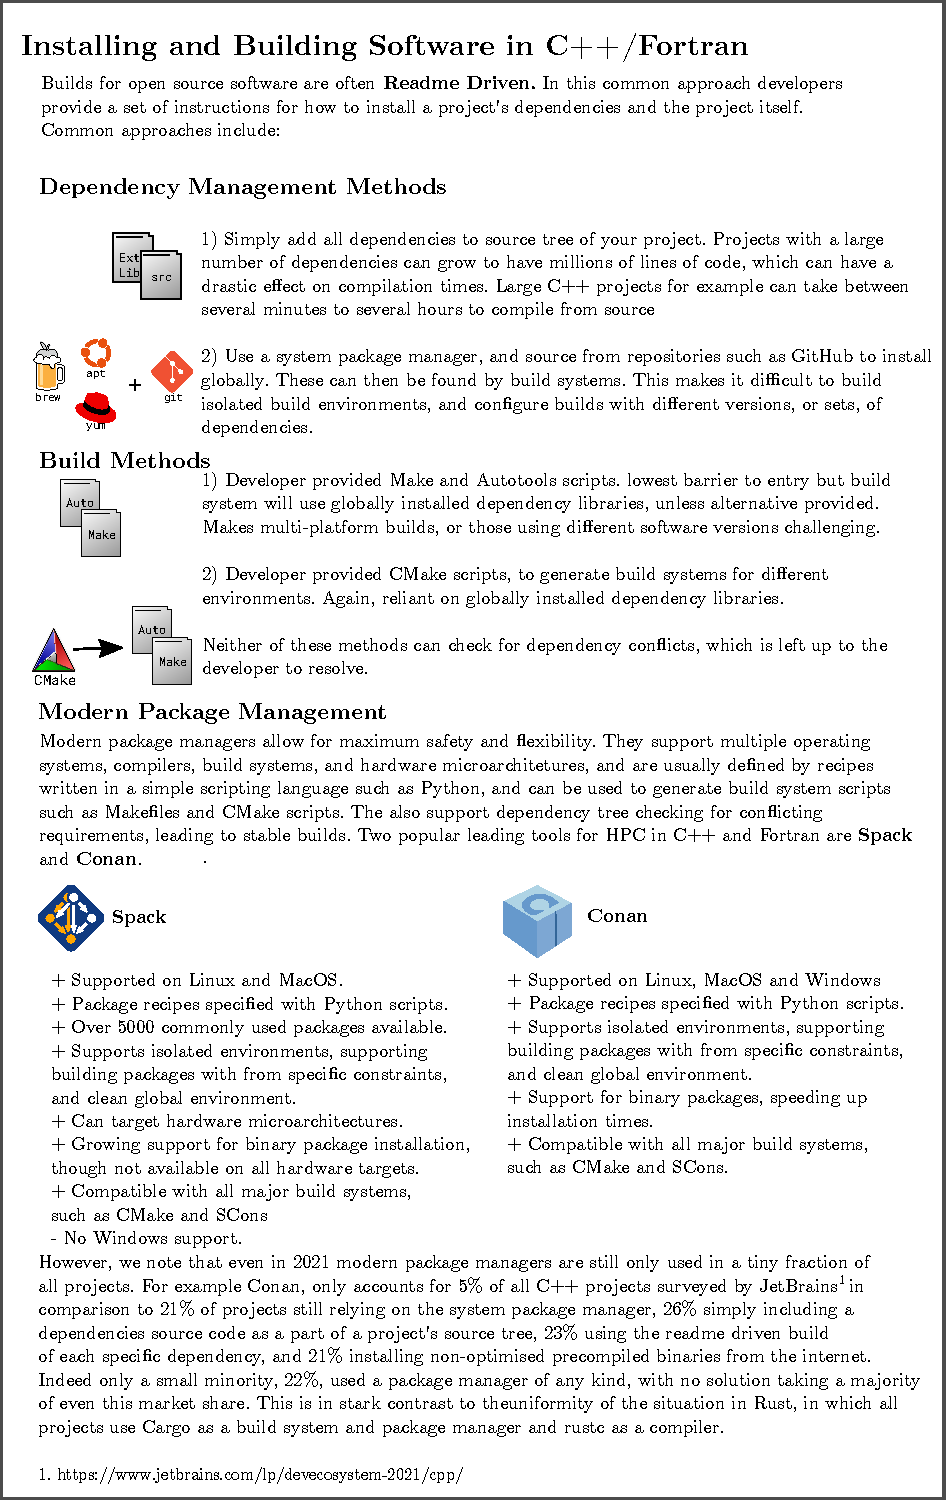
\includegraphics[width=0.95\linewidth]{ch_1/builds.pdf}}
    \caption{An overview of building software in other compiled languages.}
    \label{fig:chpt:1:sec:2:builds}
\end{figure}
